\section{Leitungstheorie}
\index{Leitungstheorie}
Ebook Strauss\\
Zur Einführung:\\
\begin{figure}[!h]
\centering
\subfloat[Schema]{
	\tikzexternaldisable
\begin{circuitikz} [scale=2, european]
	\ctikzset{bipoles/length=1.2cm}
	\draw (0,0) to [R=$50\Omega$] (1,0) to [cspst=$0$] (1.9,0) to (5,0) to [R=$25\Omega$] (5,-1)
	to (0,-1)
	(0,0) to [V=$12V$] (0,-1);
	\draw node at (2.5,-0.5) {$\underline{Z}_0 50\Omega$};
	%Spannungspfeile
	\draw [red] (2,0) to[open, v>=$\underline{U}_1$] (2,-1);
	\draw [blue] (3.5,0) to[open, v>=$\underline{U}_2$] (3.5,-1);
	\draw [green] (5,0) to[open, v>=$\underline{U}_3$] (5,-1);
	%Strompfeile
\end{circuitikz}
%\tikzexternalenable
	\label{fig:leitungstheorie:bsp1:schema}}\\
\subfloat[Spannung U]{
	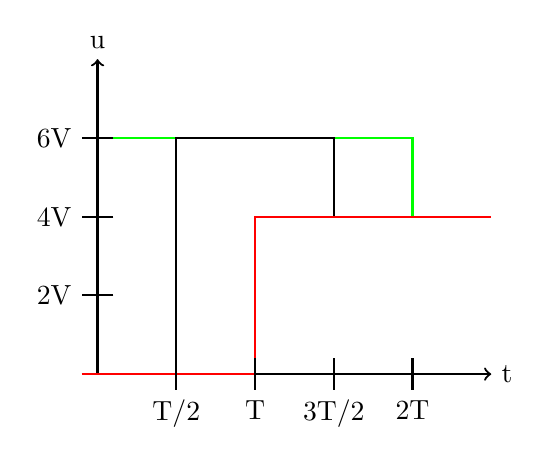
\begin{tikzpicture}[thick]
	\draw [->] (0,0) -- (5,0) node[anchor=west] {t};
	\draw [->] (0,0) -- (0,4) node[anchor=south] {u};
	\draw [green] (-0.2,3) -- (4,3) -- (4,2) -- (5,2);
	\draw [black] (-0.2,0) -- (1,0) -- (1,3) -- (3,3) -- (3,2) -- (5,2);
	\draw [red] (-0.2,0) -- (2,0) -- (2,2) -- (5,2);
	\draw (0.2,1) -- (-0.2,1) node[anchor=east] {2V};
	\draw (0.2,2) -- (-0.2,2) node[anchor=east] {4V};
	\draw (0.2,3) -- (-0.2,3) node[anchor=east] {6V};
	\draw (1,0.2) -- (1,-0.2) node[anchor=north] {T/2};
	\draw (2,0.2) -- (2,-0.2) node[anchor=north] {T};
	\draw (3,0.2) -- (3,-0.2) node[anchor=north] {3T/2};
	\draw (4,0.2) -- (4,-0.2) node[anchor=north] {2T};
\end{tikzpicture}
	\label{fig:leitungstheorie:bsp1:u}
}
\qquad
\subfloat[Strom I]{
	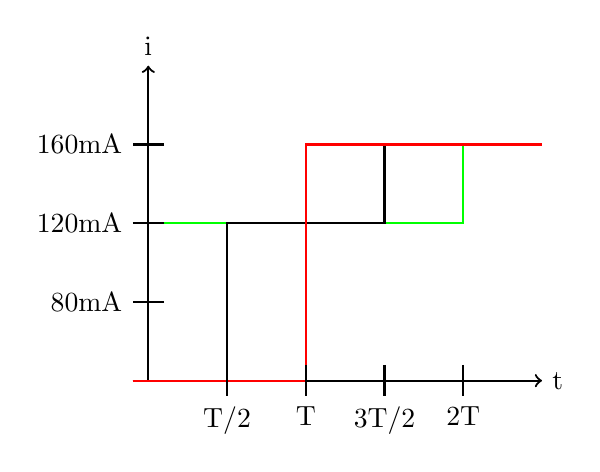
\begin{tikzpicture}[thick]
	\draw [->] (0,0) -- (5,0) node[anchor=west] {t};
	\draw [->] (0,0) -- (0,4) node[anchor=south] {i};
	\draw [green] (-0.2,2) -- (4,2) -- (4,3) -- (5,3);
	\draw [black] (-0.2,0) -- (1,0) -- (1,2) -- (3,2) -- (3,3) -- (5,3);
	\draw [red] (-0.2,0) -- (2,0) -- (2,3) -- (5,3);
	\draw (0.2,1) -- (-0.2,1) node[anchor=east] {80mA};
	\draw (0.2,2) -- (-0.2,2) node[anchor=east] {120mA};
	\draw (0.2,3) -- (-0.2,3) node[anchor=east] {160mA};
	\draw (1,0.2) -- (1,-0.2) node[anchor=north] {T/2};
	\draw (2,0.2) -- (2,-0.2) node[anchor=north] {T};
	\draw (3,0.2) -- (3,-0.2) node[anchor=north] {3T/2};
	\draw (4,0.2) -- (4,-0.2) node[anchor=north] {2T};
\end{tikzpicture}
	\label{fig:leitungstheorie:bsp1:i}
}\\
\caption{U und I im Beispiel, T ist Laufzeit für die Länge}
\label{fig:leitungstheorie:bsp}
\end{figure}
\begin{align}
	\Delta Z &= -R^\prime\cdot\Delta Z \cdot i - L^\prime\Delta Z
	\cdot \dot i\nonumber\\
	\frac{\Delta U}{\Delta Z} &= \left. -R^\prime\cdot i - L^\prime\dot i \right|
	\Delta Z \rightarrow 0\nonumber\\
	\boxed{\frac{\delta u}{\delta z}=-R^\prime i- L^\prime \frac{\delta i}{\delta
	t}}\label{leitungstheorie:wellengleichung1}
\end{align}
Korrektur Buch Seite 61, Formel 3.3, Untere Formel u durch i ersetzen\\
\begin{align}
	\Delta i &= -G^\prime \Delta Z \cdot U - C^\prime \Delta Z \cdot \dot
	U\nonumber\\
	\boxed{\frac{\delta i}{\delta Z}=-G^\prime U - C^\prime \frac{\delta u}{\delta
	t}}\label{leitungstheorie:wellengleichung2}\\
	\gamma = \sqrt{\left(R^\prime+j\omega L\right)\left(G^\prime+j\omega
	C\right)}\nonumber
\end{align}
Einsetzen, ergibt Telegrafengleichungen\\
% \begin{align}
% 	\underline{U}(z)=\underline{U}_{Vo}e^{-\underline{\gamma}
% 	z}+\underline{U}_{ro}e^{\underline{\gamma}Z}\nonumber\\
% 	\underline{I}(z)=\underline{I}_{Vo}e^{-\underline{\gamma}
% 	z}+\underline{I}_{ro}e^{\underline{\gamma}Z}\nonumber\\
% 	\underline{Z}_0=\sqrt{\frac{R^\prime+j\omega L^\prime}{G^\prime+j\omega
% 	C^\prime}}=\sqrt{\frac{Z^\prime}{C^\prime}}\nonumber
% \end{align}
% \begin{align}
% 	\frac{\delta^2u}{\delta z^2}=R^\prime G^\prime U+R^\prime C^\prime
% 	\frac{\delta u}{\delta t} +L^\prime G^\prime\frac{\delta u}{\delta t}+L^\prime
% 	C^\prime \frac{\delta^2 u}{\delta t^2}\\
% 	\frac{\delta^2i}{\delta z^2} = R^\primeG^\prime i+\left(R^\prime
% 	C^\prime+L^\prime G^\prime\right)\\
% \end{align}
Ansatz:
\begin{align}
	u(t,z) &= Re \{ \underline{\hat U}(z)\cdot e^{j\omega t} \} \nonumber\\
	u(t,z) &= Re \{ \underline{\hat I}(z)\cdot e^{j\omega t} \} \nonumber
\end{align}
angewandt auf \ref{leitungstheorie:wellengleichung1} und
\ref{leitungstheorie:wellengleichung2}\\
\begin{align}
	\frac{d\underline{U}}{dZ}=-R^\prime\cdot\underline{I}-j\omega
	L^\prime\cdot\underline{I}=- \underbrace{\left(R^\prime+j\omega
	L^\prime\right)}_{\underline{Z}^\prime=\text{Belag der
	Längsimpedanz}}\cdot\underline{I}\label{leitungstheorie:angewandt1}\\
	\frac{d\underline{I}}{dZ}=-G^\prime\cdot\underline{U}-j\omega
	C^\prime\cdot\underline{U}=- \underbrace{\left(G^\prime+j\omega
	C^\prime\right)}_{\underline{Y}^\prime=\text{Belag der
	Queradmittanz}}\cdot\underline{U}\label{leitungstheorie:angewandt2}
\end{align}
\ref{leitungstheorie:angewandt1} ableiten, \ref{leitungstheorie:angewandt2}:
\begin{align}
	\frac{d^2\underline{U}}{dz^2}&=-\left(R^\prime+j\omega
	L^\prime\right)\frac{d\underline{I}}{d\underline{Z}}\nonumber\\
	\frac{d^2\underline{U}}{dz^2}&=\underbrace{\left(R^\prime+j\omega
	L^\prime\right)}_{\underline{Z}^\prime}\underbrace{\left(G^\prime+j\omega
	C^\prime\right)}_{\underline{Y}^\prime}\underline{U}=\underline{\gamma}^2\underline{U}\label{leitungstheorie:telegrafengleichung1}\\
	\frac{d^2\underline{I}}{dz^2}&=\left(\ldots\right)\left(\ldots\right)\underline{I}=\underline{\gamma}^2\underline{I}\label{leitungstheorie:telegrafengleichung2}
\end{align}
\ref{leitungstheorie:telegrafengleichung1} und
\ref{leitungstheorie:telegrafengleichung2} sind die Telegrafengleichungen im
Frequenzbereich.\\
\begin{align}
	\frac{d^2\underline{U}(z)}{dz^2}-\underline{\gamma}^2\underline{U}(z)&=0\nonumber\\
	\underline{U}(z)&=\underline{U}\cdot e^{pt}&&\text{Ansatz, }(p \neq
	j\omega)\nonumber\\
	p^2\cdot
	\underline{U}e^{pt}-\underline{\gamma}\underline{U}e^{pt}&=0\nonumber\\
	\underline{U}e^{pt}\left(p^2-\underline{\gamma}^2\right)&=0\nonumber\\
	p^2-\underline{\gamma}^2&=0)&&\text{Charakteristische Gleichung}\nonumber\\
	p&=\sqrt{\underline{\gamma}^2}\nonumber
\end{align}
\begin{tabular}{lll}
$\gamma$ & Ausbreitungskonstante \\
$\gamma$ & $= \alpha +j\beta$ \\
$\alpha$ & Dampf.-Belag & $[\alpha]=Np/m$\\
$1Np$ & $=$1 Neper & $\mathrel{\widehat{=}}$ Dämpfung um Faktor
$e^1=2.718\mathrel{\widehat{=}}8.686dB$\\
$\beta$ & Phasenbelag & $[\beta]=rad/m$\\
\end{tabular}

\begin{align}
	\underline{U}(z) &= \underline{U}_{V0}\cdot e^{-\underline{\gamma}
	z}+\underline{U}_{r0}\cdot
	e^{\underline{\gamma}z}=\underline{U}_v(z)+\underline{U}_r(z)\nonumber\\
	%Links vom + gelb unterstrichen, rechts blau
	&= \underline{U}_{vo}\cdot e^{-\alpha z}\cdot e^{-j\beta
	z}+\underline{U}_{r0}\cdot e^{\alpha z}\cdot e^{j\beta z}\nonumber
\end{align}
Bild 1 Bild 2\\
Eine Umdrehung des Zeigers entspricht einer Wellenlänge $\lambda$\\
\begin{align}
	\Rightarrow \beta z = \beta \lambda = 2 \pi\nonumber\\
	\boxed{\beta=\frac{2\pi}{\lambda}}\nonumber
\end{align}
\textbf{Zurück in den Zeitbereich}
\begin{align}
	u(t,z)&=Re\{\hat{\underline{U}}(z)\cdot e^{j\omega t}\nonumber\\
	%links gelb, rechts vom + blau
	&=Re\{\hat{\underline{U}}_{v0}e^{-\underline{\gamma}z}e^{j\omega
	t}\}+Re\{\hat{\underline{U}}_{r0}e^{\underline{\gamma}z}e^{j\omega
	t}\}\nonumber\\
	U_v(t,z)&=Re\{\underline{\hat{U}}_{v0}\cdot e^{j\varphi_v}\cdot e^{-\alpha
	z}\cdot e^{-j\beta z}\cdot e^{j\omega t}\}\nonumber\\
	%gelb boxed:
	U_v&=\hat{U}_{v0}\cdot e^{-\alpha z}\cdot \cos\left(\omega t-\beta
	z+\varphi_v\right)\nonumber
\end{align}
Bild 3\\
Wie schnell kommt die Welle vorwärts?\\
$\omega t-\beta Z=konst$ (d.h. konstanter Winkel in der cos-Funktion)\\
$\omega\Delta T=\beta\Delta Z$\\
%blau boxed:
$v_p=\frac{\Delta Z}{\Delta t}=\frac{\omega}{\beta}$\\
Skript Seite 64\\
dazu: falls $v=konst. v=\frac{\omega}{\beta}\Rightarrow \omega=v\beta$\\
Bild 4\\
\subsection{Reflexionsfaktor r}
Skript Seite 67\\
Bild 5\\
Am Leitungsende:\\
\begin{align}
	\underline{U}&=\underline{I}\cdot\underline{Z}_E\nonumber\\
	\underline{U}&=\underline{U}_v+\underline{U}_r=\left(\underline{I}_v-\underline{I}_r\right)\cdot\underline{Z}_E\nonumber\\
	\underline{U}_v+\underline{U}_r&=\frac{\underline{Z}_E}{\underline{Z}_0}\left(\underline{U}_v-\underline{U}_r\right)\nonumber\\
	\underline{U}_r\left(1+\frac{\underline{Z}_e}{\underline{Z}_0}\right)&s=\underline{U}_v\left(\frac{\underline{Z}_e}{\underline{Z}_0}-1\right)\nonumber\\
	\underline{r}_E=\frac{\underline{U}_r}{\underline{U}_v}&=\frac{\frac{\underline{Z}_e}{\underline{Z}_0}-1}{\frac{\underline{Z}_e}{\underline{Z}_0}+1}=\frac{\underline{Z}_E-\underline{Z}_0}{\underline{Z}_E+\underline{Z}_0}\nonumber\\
	\text{falls: }\underline{Z}_E=R, \underline{Z}_0&=R_0
	\boxed{r=\frac{R-R_0}{R+R_0}}\nonumber
\end{align}
Skript Seite 68 ff\\
\begin{align}
	\underline{r}_A&=\frac{\underline{U}_{Ar}}{\underline{U}_{Av}}=\frac{\underline{U}_{Er}\cdot
	e^{-\underline{\gamma}  l}}{\underline{U}_{Ev}\cdot e^{\underline{\gamma}
	l}}=\boxed{\underline{r}_E\cdot e^{-2\underline{\gamma}l}}\nonumber
\end{align}
343: $\underline{Z}=\underline{Z}_0\frac{1+r}{1-r}$
